\section{Receive Input}

The receive input interface takes packets from the receive interface
of the GMII and places them into the FIFO, checking for both RX fifo
overflow and verifying the FCS.

\subsection{Interface}
The input here is the GMII interface from the Ethernet PHY. The output
data is written to the RX FIFO by setting \signal{MA[15:0]} and
\signal{MD[31:0]} for four cycles to guarantee latching. The
\signal{BPOUT[15:0]} points to the base of the
next-packet-to-be-written.

The module takes in a series of signals from the control interface to
evaluate whether or not we are the intended recipient for a given
frame. See the implementation the RX Valid module for further details. 

If the received frame has a valid CRC, that frame and its FCS are
written into the RX FIFO. Thus we again suffix every RAM FIFO write
with a CRC.


\subsection{Implementation}

There are three additional submodules that comprise the receive interface. 

\subsubsection{GMIIin}
\import{.}{gmiiin.tex}

\subsubsection{RX Packet FIFO} 
\import{.}{rxpktfifo.tex}

\subsubsection{RX Valid}
\import{.}{rxvalid.tex}


\subsubsection{Combining it all}
The included FSM reads a single packet at a time out of the RX Packet
FIFO by asserting \signal{NEXTF}. After verifying and discarding the
preamble, we acquire each byte and selectively write it to the
\signal{LM[31:0]} word.


\begin{figure}
\label{rxinput}
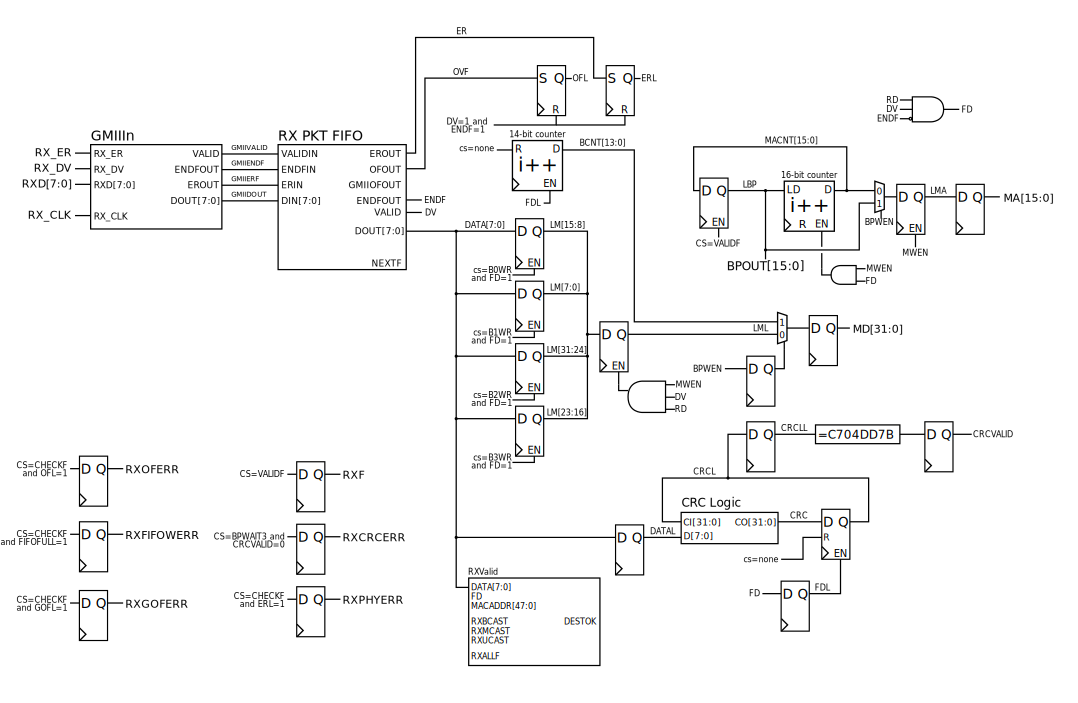
\includegraphics[scale=0.7]{rxinput.svg}
\caption{The RX Input, verifying correct packets}

\end{figure}

\begin{figure}
\label{rxinputfsm}
\includegraphics[scale=0.7]{rxinput.fsm.svg}
\caption{The RX Input FSM, verifying correct packets}
\end{figure}

